\appendix
\section*{Appendix}

\section{Public Release of Codebase and Detail Prompts}
We plan to gradually release a codebase. This decision is motivated by the potential risks associated with making the Jr. AI Scientist easy to use. 
As discussed in the main paper, AI Scientist systems, including the Jr. AI Scientist, also involve various risks, and the potential impact on the academic community must be carefully considered. Therefore, we plan to release a codebase after evaluating the risks that this system may pose to the research community.


\section{Main Prompts for Jr. AI Scientist}
An example of the prompt in the Idea Generation Phase is shown below.
Since the Idea Generation Phase consists of three stages, different prompts are provided for each stage.
\subsection{Idea Generation}
%%% 
%%% PAPER TEXTの説明を追加する?
%%%
\begin{tcolorbox}[colback=gray!10, colframe=gray!40!black, breakable=true, title=Prompt for Limitation Analysis]
    Please analyze the following paper text and identify limitations (constraints/challenges) from a broad perspective.

Paper Text:
\textbf{\{PAPER TEXT\}}\\

Please analyze limitations from the following perspectives:\\
1. Method/Algorithm limitations\\

For each limitation:\\
- Explain the specific problem\\
- Explain why it is problematic\\
- Propose improvement directions\\

Additional Requirement:\\
- Include the perspective of "AI autonomously conducting research". 
  You may assume that the AI is provided with access to the codebase of this research. 
  For each limitation, explain how an autonomous AI research agent could 
  refine this limitation through self-experiments, 
  automated ablation, or meta-learning.

Constraints:\\
- Focus on limitations that can be addressed through relatively simple implementation changes 
  but would have significant impact if improved.\\
- Do not focus too much on innovativeness; instead, identify limitations with substantial potential for solid performance improvement.\\
- Output the analysis in a structured format.\\

Output Structure:\\
\#\# Method/Algorithm Limitations

\#\#\# Limitation 1: [Short Title]\\
- Specific Problem: ...\\
- Why Problematic: ...\\
- Improvement Directions:\\
  - [Simple fix or adjustment]\\
  - [Autonomous AI research perspective]\\

\#\#\# Limitation 2: [Short Title]\\
...

\#\#\# Limitation 3: [Short Title]\\
...
\end{tcolorbox}


%%% 
%%% PAPER TEXT, LIMITATION, PREV IDEAS の説明を追加
%%%
\begin{tcolorbox}[colback=gray!10, colframe=gray!40!black, breakable=true, title=Prompt for Idea Generation]
Please generate one new research idea based on the following paper limitation analysis.\\

Original Paper:
\textbf{\{PAPER TEXT\}}\\

Limitation Analysis:
\textbf{\{LIMITATIONS\}}\\

Already generated ideas:
\textbf{\{PREV IDEAS\}}\\

Constraints:\\
1. The proposal should not require large computational resources or extensive data collection.\\
2. Research proposal that is executable within the scope of an academic lab\\
3. Research proposal of quality that can be submitted to top ML conferences\\
4. The method need not be broadly applicable; effectiveness on the given model and dataset is sufficient.\\
5. Aim for a simple, effective implementation rather than a complex or overly innovative one.\\
6. Do not focus too much on innovativeness; instead, propose a method with solid performance improvement.\\
7. This research should be conducted by an autonomous AI agent, 
   which means human research activities (e.g., human-in-the-loop) should be excluded.\\

Please generate one research idea in the following format. Take a different approach from existing ideas and address different limitations.\\

**Important**: Always respond in the following JSON format. Include ```json.\\

\begin{verbatim}
```json
{
  "idea": {
    "Name": "Short name for research idea (lowercase, underscores allowed)",
    "Title": "Catchy and informative title",
    "Short Hypothesis": "Concise explanation of main hypothesis or research question. 
Clearly explain why this direction is needed, confirm that this setting is optimal
for investigating this idea, and confirm that there are no other obviously simpler
ways to answer the question.",
    "Related Work": "Brief discussion of most relevant related work and how the
proposal clearly distinguishes from them, and is not a trivial extension.",
    "Abstract": "Conference format proposal summary (approximately 250 words)",
    "Experiments": "List of experiments to be conducted to validate the proposal.
Ensure these are simple and feasible. Explain specifically how you would test the
hypothesis and detail precise algorithmic changes. Include evaluation metrics
you would use.",
    "Risk Factors and Limitations": "List of potential risks and limitations of the
proposal"
}
}
'''
\end{verbatim}

\end{tcolorbox}




\subsection{Experimentation}
\label{appendix:experimentation}
% \begin{comment}
% 実験に必要なコードを書かせるために、Coding Agentに与えるプロンプトの例を以下に示す。
% Experiment Phaseでは4つのステージがあるためそれぞれのステージで異なったプロンプトが与えられる。
% さらに一つのステージの中でもエージェントの実行毎にMEMORYなどの要素は少しずつ異なり得る。
% \begin{itemize}
% \item ``introduction''、``directory\_structure''、``research\_idea''要素は全てのステージで共通である。
% \item ``research\_idea'' にはIdea Generation Phase で生成した研究アイデアが直接挿入され、今から実装する機能の俯瞰的なコンテキストをCoding Agentに与える。例をプロンプトの後に示す。
% \item Stage2と Stage3・4 ではそれぞれ``performance\_improvement\_idea''と``ablation\_study\_idea''が挿入される。これは実装方針となるアイデアであり、例を続けて示す。
% \item ``memory''にはこれまでそのStageで行われた実験についてのサマリーが埋め込まれる。成功した実験の結果およびメトリクス、失敗した実験の原因およびエラーログなどを用いてLLMがようやくしたものが埋め込まれる。``memory''の例については長くなるため、一部省略し後に示す。
% \item ``required\_functionality''に、Coding Agentが実装すべき主な機能が記載されている。この内容はステージごとに短い説明文とエントリポイントとなるファイル名だけが異なる。Stage1では提案手法の実装を行うため``proposed\_method\_implementation''となる。Stage2では提案手法の精度改善を行うため要求する実装機能としては``improved\_proposed\_method''となる。
% \end{itemize}
% \end{comment}
An example of the prompt given to the Coding Agent to make it write the code required for the Experiment Phase is shown below.
Since the Experiment Phase consists of four stages, different prompts are provided for each stage.
In addition, even within the same stage, elements such as <memory> may vary slightly across different executions of the agent.

\begin{itemize}
\item The <introduction>, <directory\_structure>, and <research\_idea> elements are shared across all stages.
\item The <research\_idea> directly contains the research idea generated in the Idea Generation Phase, providing the Coding Agent with a high-level contextual overview of the functionality to be implemented.
\item In Stage 2 and Stages 3–4, <performance\_improvement\_idea> and <ablation\_study\_idea> are inserted, respectively. These guide the implementation strategy.
\item The <memory> field embeds a summary of the experiments conducted so far within the corresponding stage. This includes results and metrics from successful experiments, as well as causes of failed experiments and error logs, summarized by the LLM.
\item The <required\_functionality> specifies the main functionalities that the Coding Agent is expected to implement. While this content differs across stages, the differences are limited to a short descriptive text and the name of the entry-point file. In Stage 1, where the proposed method is implemented, this field is set to <proposed\_method\_implementation>. In Stage 2, which focuses on improving the performance of the proposed method, the required functionality is specified as <improved\_proposed\_method>.
\end{itemize}

%%%
%%% BASE PROMPT
%%%
\begin{tcolorbox}[colback=gray!10, colframe=gray!40!black, breakable=true, title=Prompt for Coding Agent (An Example in Stage 1)]
<introduction>\\
You are an experienced AI researcher.\\
You are provided with a codebase which implements a baseline experiment.\\
Follow the instructions below and modify the code as necessary.\\
</introduction>
\vspace{6pt}

<directory\_structure>\\
<baseline.py>\\
A python script that runs the baseline experiment.\\
- Don't modify this file because it works fine.\\
Args:\\
- \text{-}-output-dir (str): path to the output directory where results will be saved.\\
</baseline.py>
\vspace{6pt}

<plot.py>\\
- A python script that generates plots for the experimental results.\\
- Don't modify this file because it works fine\\
- This script loads `scores.npz` file and plots the score distributions.\\
- All experimental results, including ablation studies, must be plotted using this script; do not write a separate plotting script.\\
Args:\\
- \text{-}-input-file (str): path to the input `scores.npz` file.\\
- \text{-}-output-dir (str): path to the output directory where plots will be saved.\\
</plot.py>
\vspace{6pt}

<baseline\_code\_dir>\\
This directory is the original baseline code directory.\\
- Don't modify this directory. You should keep this directory as it is.\\
- This directory contains the baseline code.\\
- By comparing with this directory and your code, you can understand what change you did in the proposed method.\\
</baseline\_code\_dir>
\vspace{6pt}

</directory\_structure>
\vspace{6pt}

<research\_idea>\\
\textbf{\{RESEARCH IDEA\}}\\
</research\_idea>
\vspace{6pt}

<performance\_improvement\_idea>\\
\textbf{\{PERFORMANCE IMPROVEMENT IDEA\}}\\
</performance\_improvement\_idea>
\vspace{6pt}

<ablation\_study\_idea>\\
\textbf{\{ABLATION STUDY IDEA\}}\\
</ablation\_study\_idea>
\vspace{6pt}

<memory>\\
\textbf{\{MEMORY\}}\\
</memory>
\vspace{6pt}

<required\_functionality>\\
<proposed\_method\_implementation>\\
You implement the proposed method based on research idea exploring novel improvements or revealing new insights.\\
- You should implement only the core part of the idea, without changing the input/output file formats.\\
- The entry script must take the same arguments as baseline.py and produce output files.\\
- The output file schema (npz, json) must also be the same as in baseline.py.\\
- Keep codebase modifications to a minimum, except where changes are necessary to implement the idea.\\
- The entry script must be named proposed\_method.py.\\
Example:\\
\verb|```|\\
python proposed\_method.py \text{-}-output-dir .\/results\\
\verb|```|\\
<important\_notes>\\
Write implementation plan in plan\_proposed\_method.md file.\\
</important\_notes>
\vspace{6pt}

</proposed\_method\_implementation>
\vspace{6pt}

</required\_functionality>
\vspace{6pt}

<dataset\_directory>\\
The necessary datasets are stored in the following directory: /datasets/LoCoOp.\\
No additional datasets should be downloaded.\\
</dataset\_directory>
\end{tcolorbox}



\subsection{Writing}
The prompt used for Draft Writing in the Writing Phase is shown below.
The portion denoted as \{RESEARCH IDEA\} is identical to the text presented in \ref{appendix:experimentation}.
\{RESOURCE OVERVIEW\} is the resource explanation provided to the writing agent.
\{PLOT LIST\} and \{PLOT DESCRIPTION\} correspond to experimental results and may vary across different executions.

%%%
%%% DETAILED WRITING
%%%
\begin{tcolorbox}[colback=gray!10, colframe=gray!40!black, breakable=true, title=Prompt for Detailed Writing]
Your goal is to write up the following idea:\\
\\
\verb|```|markdown\\
\textbf{\{RESEARCH IDEA\}}\\
\verb|```|\\
Note that idea\_text represents a preliminary hypothesis and may not necessarily align with the experiments that were eventually performed.\\
\\
First, make sure to refer to the experiment summaries contained in baseline\_summary.json, improved\_research\_summary.json, hyperparam\_ablation\_summary.json and component\_ablation\_summary.json.
Important: The experiment results in hyperparam\_ablation\_summary.json and component\_ablation\_summary.json are summarized in the tables hyperparam\_ablation\_summary\_table.tex and component\_ablation\_summary\_table.tex. 
In these .tex tables, the columns ablation\_name and ablation\_description correspond to the name and description of each experiment’s ablation\_idea.
Do not directly copy these descriptions into the .tex tables. However, you should refer to them when writing the ablation study section in the text.
You may modify how the non-numerical content is written in the .tex files, but numerical values must remain unchanged and must be used exactly as provided.\\
(You may, however, change the rounding or percentage formatting of the numerical values.)\\
\\
Available plots for the writeup (use these filenames):\\
\verb|```|\\
\textbf{\{PLOT LIST\}}\\
\verb|```|\\

Please also consider which plots can naturally be grouped together as subfigures.\\

We also have VLM-based figure descriptions:\\
\verb|```|\\
\textbf{\{PLOT DESCRIPTION\}}\\
\verb|```|\\

To better understand the methodology, please also refer to:\\
\textbf{\{RESOURCE OVERVIEW\}}\\
% - baseline\_tex/ and baseline\_code/baseline.py as the baseline TeX and code, respectively. When writing up the baseline method, you must follow its method section.\\
% - baseline\_tex/baseline\_bibtex.txt contains the baseline paper's bibliographic information and title - read this file to identify the baseline method being compared against.\\
% - proposed\_method\_code/improved\_proposed\_method.py as the proposed method's code implementation (note that the proposed method should be referenced in improved\_proposed\_method.py rather than proposed\_method.py)\\
% - method\_section.tex (pre-written Method section with detailed technical analysis)\\
\\
Please read the current template.tex file and update it to produce a complete, coherent, and scientifically accurate paper.\\
This must be an acceptable complete LaTeX writeup, suitable for a 8-page single-column paper.\\
Make sure to use the citations from the references.bib file and report results accurately based on the experimental data provided.\\
Start by reading template.tex to understand the current state, then edit it to incorporate all the information above into a complete paper.\\
\\
Please note: For the bibliography, do not use the \verb|\|begin\{filecontents\}\{references.bib\} environment. Instead, all citations should refer to an external file named references.bib.\\
\\
Please use the structure plan saved in paper\_structure.md as guidance for writing the full paper.
\end{tcolorbox}


%%%
%%% CITATION VALIDATION
%%%
\begin{tcolorbox}[colback=gray!10, colframe=gray!40!black, breakable=true, title=Prompt for Citation Validation]
Your task is to validate and improve the citations in the paper, particularly in the Related Work section, by comparing with a high-quality baseline paper.\\

Research idea:\\
\verb|```|markdown\\
\textbf{\{RESEARCH IDEA\}}\\
\verb|```|\\

Note that idea\_text represents a preliminary hypothesis and may not necessarily align with the experiments that were eventually performed.\\

Please perform the following steps:\\

1. **Analyze Citation Standards from Baseline Paper:**\\
   - Read a paper from baseline\_tex/ to understand the citation standards in this field\\
   - Pay attention to:\\
     - The typical number of citations per section\\
     - How citations are grouped and discussed thematically\\
     - The balance between classic/foundational papers and recent work\\
     - Citation density in the Related Work section\\
\\
2. **Evaluate Current Citations:**\\
   - Read the current template.tex file\\
   - Count the total number of unique citations\\
   - Analyze citation distribution across sections\\
   - Check if all citations in references.bib are actually used\\
\\
3. **Identify Citation Gaps:**\\
   - Compare your citation count and distribution with the baseline papers\\
   - Identify areas where additional citations would strengthen the paper\\
   - Check if any important research areas or foundational works are missing\\
\\
4. **Improve Citations:**\\
   - Add citations where the paper makes claims that should be supported\\
   - Ensure the Related Work section has comprehensive coverage\\
   - Make sure recent relevant work (within last 3-5 years) is adequately cited\\
   - Verify that seminal/foundational papers in the field are included\\
\\
5. **Citation Quality Check:**\\
   - Ensure citations are properly formatted and consistent\\
   - Check that each citation adds value and is discussed meaningfully\\
   - Avoid citation padding - each citation should serve a clear purpose\\
\\
Please use the Read, Edit, and MultiEdit tools to:\\
- First analyze baseline\_tex/ papers to understand citation standards\\
- Then review and improve the citations in template.tex\\
- Focus especially on the Related Work section but also check other sections\\
\\
After your analysis, make the necessary edits to improve the citation quality and coverage to match the standards of the field.\\
\\
Please note: For the bibliography, do not use the \verb|\|begin\{filecontents\}\{references.bib\} environment. Instead, all citations should refer to an external file named references.bib.
\end{tcolorbox}


\begin{comment}
続けて、Reflectionで使用するプロンプトを以下に示す。
\end{comment}
Next, we present the prompt used for Reflection.

%%%
%%% FEEDBACK GENERATION
%%%
\begin{tcolorbox}[colback=gray!10, colframe=gray!40!black, breakable=true, title=Prompt for Feedback Generation]
\# Role
You are an AI assistant specializing in reviewing scientific manuscripts. Your mission is to analyze the provided artifacts (manuscript, data, code, etc.) from multiple angles and generate precise, constructive feedback based on the specified criteria.\\

\# Instructions\\
Read the content from the provided file paths and information, then generate a feedback report that focuses on the following criteria. For each criterion, state clearly if no issues are found, or provide specific details if problems or potential improvements are identified.\\

\# Feedback Criteria\\
1.  **Verification for Falsification \& Inconsistency:**\\
    * Thoroughly cross-reference the claims made in the manuscript ./template.tex — including text, tables, and figures—against objective evidence from Experiment Summaries (JSON format), proposed\_method\_code/improved\_proposed\_method.py, and Plot Descriptions (from VLM). **Treat the Research Idea as background context only and do not flag discrepancies between it and the final manuscript.**\\
    * Identify and report all suspected inconsistencies, such as numerical mismatches, discrepancies between the described methodology and the source code logic, and biased interpretations of plots. **All numerical discrepancies resulting from rounding are to be ignored.**\\
\\
2.  **Verification for Guideline Adherence:**\\
    * Check if the manuscript complies with the rules and guidelines provided in CLAUDE.MD file.\\
    * Report any deviations from the guidelines, including issues with formatting, style, mathematical notation, or section structure.\\
\\
3.  **Verification for Missing Citations:**\\
    * Examine the manuscript for claims that require a citation but lack one, particularly for background concepts, related work, and datasets.\\
    * Using the content from ./template.tex as a reference, suggest specific citations that should be added.\\
    * **For each missing citation, create a descriptive string that clearly identifies the paper to be found (e.g., 'The original Transformer paper, ``Attention Is All You Need.'' '). These descriptions will form a list to be saved in a single JSON file.**\\
\\
4.  **Suggestions for Section-by-Section Improvements:**\\
    * For each major section of the manuscript (Abstract, Introduction, Method, Experiments, Conclusion, etc.), propose concrete improvements to enhance clarity, persuasiveness, and impact.\\
    * Provide actionable advice on aspects like logical flow, readability, and the effective use of figures and tables.\\
    * Please ensure that all suggestions are actionable within the scope of the provided experiments and code, without requiring new experimental runs.\\
    * Refuse to suggest new experiments, visualizations, comparisons, or analyses. All suggestions must be limited to encouraging deeper discussion based on the provided text, figures, and existing data.\\
    * Focus on suggestions that amplify the manuscript's strengths and maximize the impact of its contributions. Instead of flagging claims as overstated, suggest how to rephrase or restructure the narrative to make them more compelling based on the existing evidence.**\\
\\
\# Inputs\\
\#\# Research Idea:\\
\verb|```|markdown\\
\textbf{\{RESEARCH IDEA\}}\\
\verb|```|\\

Note that idea\_text represents a preliminary hypothesis and may not necessarily align with the experiments that were eventually performed.\\

\#\# Experiment Summaries (JSON format)\\
Refer to the experiment summaries contained in baseline\_summary.json, improved\_research\_summary.json, hyperparam\_ablation\_summary.json and component\_ablation\_summary.json.\\
Important: The experiment results in hyperparam\_ablation\_summary.json and component\_ablation\_summary.json are summarized in the tables hyperparam\_ablation\_summary\_table.tex and component\_ablation\_summary\_table.tex. \\
In these .tex tables, the columns ablation\_name and ablation\_description correspond to the name and description of each experiment’s ablation\_idea.\\
Do not directly copy these descriptions into the .tex tables. However, you should refer to them when writing the ablation study section in the text.\\
You may modify how the non-numerical content is written in the .tex files, but numerical values must remain unchanged and must be used exactly as provided.\\
(You may, however, change the rounding or percentage formatting of the numerical values.)\\

\#\# Available Plots (list of filenames)\\
\verb|```|\\
\textbf{\{PLOT LIST\}}\\
\verb|```|\\

\#\# Plot Descriptions (from VLM)\\
\verb|```|\\
\textbf{\{PLOT DESCRIPTION\}}\\
\verb|```|\\

To better understand the idea, experiments, and results, please also refer to:\\
- baseline\_tex/ and baseline\_code/baseline.py as the baseline TeX and code, respectively. When writing up the baseline method, you must follow its method section.\\
- baseline\_tex/baseline\_bibtex.txt contains the baseline paper's bibliographic information and title - read this file to identify the baseline method being compared against.\\
- proposed\_method\_code/improved\_proposed\_method.py as the proposed method's code implementation (note that the proposed method should be referenced in improved\_proposed\_method.py rather than proposed\_method.py)\\
- method\_section.tex (pre-written Method section with detailed technical analysis)\\

\# Output Generation\\
Based on your review, generate the following two files.\\

\verb|---|\\
\#\# Part 1: Feedback Report (Markdown)\\
- **File to Generate:** `reflection\_1\_feedback.md`\\
- **Format:** Markdown\\
- **Content:** A comprehensive report detailing the findings from all four criteria of the `Core Task`.\\

\#\#\# Markdown Report Template\\

\#\#\# 1. Results of Falsification \& Inconsistency Check\\
- [ ] No significant inconsistencies or signs of falsification were found.\\
- [ ] The following discrepancies or concerns were identified:\\
    - (e.g., Table 1 reports an accuracy of 92.5\%, but the JSON data shows an average of 91.8\%. This suggests a potential cherry-picking of the best seed's result.)\\
    - (e.g., The text describes the result in Figure 3 as a ``significant improvement,'' but comparison with the VLM description indicates it is within the margin of error. The claim is overstated.)\\
    - (e.g., The method section states a dropout rate of 0.5, but the implementation in the source code uses 0.3.)\\

\#\#\# 2. Results of Guideline Adherence Check\\
- [ ] The manuscript generally adheres to the provided guidelines.\\
- [ ] The following deviations from the guidelines were found:\\
    - (e.g., The font used for equations is inconsistent. Please follow the instructions in CLAUDE.md.)\\
    - (e.g., The rule that figure captions must be placed below the figure has not been followed.)\\

\#\#\# 3. Results of Missing Citations Check\\
- [ ] No significant missing citations were identified.\\
- [ ] The following sections may require additional citations:\\
    - (e.g., The second paragraph of the Introduction discusses the basic Transformer architecture but lacks a citation to the original paper, ``Attention Is All You Need.'')\\
    - (e.g., A citation should be added for the iNaturalist dataset used in the experiments, referencing the paper that introduced it.)\\

\#\#\# 4. Section-by-Section Improvement Suggestions\\
- **Abstract:** (e.g., The background description is currently too long. The abstract would be more impactful if it started with a concise one-sentence summary of the contribution and included key quantitative results.)\\
- **Introduction:** (e.g., The problem statement is clear, but the motivation could be strengthened by better explaining why this problem is important and what the broader impact of solving it would be.)\\
- **Related Work:** (e.g., Rather than simply listing prior studies, structure the section thematically. Clearly explaining how your work differs from or builds upon key papers will better highlight your unique contribution.)\\
- **Method:** (e.g., The pseudocode in Algorithm 1 is dense. Consider simplifying it to show only the main steps and moving detailed explanations to the main text to improve readability.)\\
- **Experimental Setup:** (e.g., For reproducibility, it would be beneficial to include a table summarizing all key hyperparameters. Justifying the choice of evaluation metrics and baselines would also strengthen the paper's credibility.)\\
- **Experiments:** (e.g., Instead of just listing results, add more analysis immediately after each result to discuss *why* it occurred. This would add significant depth to the paper.)\\
- **Ablation Study:** (e.g., It's unclear which components of your method contribute most to the performance gain. An ablation study that systematically analyzes the impact of each component would provide valuable insights and strengthen your claims.)\\
- **Conclusion:** (e.g., Providing more specific details on the study's limitations and future directions would demonstrate scientific rigor and foresight.)\\

\verb|---|\\
\#\# Part 2: Required Citations List (JSON)\\
- **File to Generate:** `reflection\_1\_required\_bib.json`\\
- **Format:** JSON (A list of strings)\\
- **Content:** A machine-readable list of the descriptive strings for each missing citation identified in `Core Task 3`. Each string in the list should be a clear instruction for a search tool.\\

\#\#\# JSON Format Example\\
\verb|```|json\\
\verb|[|\\
  ``The original Transformer paper, 'Attention Is All You Need' by Vaswani et al.'',\\
  ``The paper that introduced the iNaturalist dataset.''\\
\verb|]|
\end{tcolorbox}

%%%
%%% FEEDBACK REVISION
%%%
\begin{tcolorbox}[colback=gray!10, colframe=gray!40!black, breakable=true, title=Prompt for Feedback Revision]
\# Role\\
You are an expert writing assistant who accurately incorporates feedback to improve a manuscript. Your task is to faithfully execute the requested revisions to enhance the overall quality of the text.\\

\# Instructions\\
Revise the ./template.tex strictly according to the contents of the Feedback Report found at reflection\_1\_feedback.md.
Implement all the changes and suggestions noted in the feedback and output the complete, revised manuscript. Do not introduce new information or interpretations that are not specified in the feedback.
When the feedback points out missing citations, you must add appropriate \verb|\|citep\{\} commands in the main text. Refer to the Newly Acquired Citations (BibTeX format).\\

**Requests Beyond the Scope of Existing Data (CRITICAL):**\\
* If a feedback requests a new experiment, a comparison with data you do not have, or an analysis that is impossible with the provided information, **DO NOT INVENT DATA OR RESULTS.**\\
* Instead, address the comment *in the manuscript's text* by:\\
    * **First, attempting to reframe the point as a strength or a deliberate choice using the principles in Strategy \#5. As a last resort, if this is not feasible, proceed by:**\\
    * Acknowledging the value and validity of the feedback's suggestion.\\
    * Politely stating that it falls outside the scope of the current study's experiments.\\

\# Inputs\\
\#\# Research Idea:\\
\verb|```|markdown\\
\textbf{\{RESEARCH IDEA\}}\\
\verb|```|\\
Note that idea\_text represents a preliminary hypothesis and may not necessarily align with the experiments that were eventually performed.\\

\#\# Experiment Summaries (JSON format)\\
Refer to the experiment summaries contained in baseline\_summary.json, improved\_research\_summary.json, hyperparam\_ablation\_summary.json and component\_ablation\_summary.json.\\
Important: The experiment results in hyperparam\_ablation\_summary.json and component\_ablation\_summary.json are summarized in the tables hyperparam\_ablation\_summary\_table.tex and component\_ablation\_summary\_table.tex. \\
In these .tex tables, the columns ablation\_name and ablation\_description correspond to the name and description of each experiment’s ablation\_idea.\\
Do not directly copy these descriptions into the .tex tables. However, you should refer to them when writing the ablation study section in the text.\\
You may modify how the non-numerical content is written in the .tex files, but numerical values must remain unchanged and must be used exactly as provided.\\
(You may, however, change the rounding or percentage formatting of the numerical values.)\\

\#\# Available Plots (list of filenames)\\
\verb|```|\\
\textbf{\{PLOT LIST\}}\\
\verb|```|\\

\#\# Plot Descriptions (from VLM)\\
\verb|```|\\
\textbf{\{PLOT DESCRIPTION\}}\\
\verb|```|

\#\# Newly Acquired Citations (BibTeX format)\\

To better understand the idea, experiments, and results, please also refer to:\\
- baseline\_tex/ and baseline\_code/baseline.py as the baseline TeX and code, respectively. When writing up the baseline method, you must follow its method section.\\
- baseline\_tex/baseline\_bibtex.txt contains the baseline paper's bibliographic information and title - read this file to identify the baseline method being compared against.\\
- proposed\_method\_code/improved\_proposed\_method.py as the proposed method's code implementation (note that the proposed method should be referenced in improved\_proposed\_method.py rather than proposed\_method.py)\\
- method\_section.tex (pre-written Method section with detailed technical analysis)\\

Please note: For the bibliography, do not use the \verb|\|begin\{filecontents\}\{references.bib\} environment. Instead, all citations should refer to an external file named references.bib.
\end{tcolorbox}

\begin{tcolorbox}[colback=gray!10, colframe=gray!40!black, breakable=true, title=CLAUDE.md for the writing agent]
You are an ambitious AI researcher who is looking to publish a paper that will contribute significantly to the field.\\
Ensure that the paper is scientifically accurate, objective, and truthful. Accurately report the experimental results, even if they are negative or inconclusive.\\
You are planning to submit to a top-tier ML conference, which has guidelines:\\
- The main paper is limited to 8 pages, including all figures and tables, but excluding references, the impact statement, and optional appendices. In general, try to use the available space and include all relevant information.\\
- The main paper should be single-column format, while the appendices can be in single-column format. When in single column format, make sure that tables and figures are correctly placed.\\
- Do not change the overall style which is mandated by the conference. Keep to the current method of including the references.bib file.\\
- Do not remove the \\graphicspath directive or no figures will be found.\\
- Do not add `Acknowledgements` section to the paper.\\
- Use a single backslash (\textbackslash) for LaTeX commands instead of a double backslash (\textbackslash\textbackslash).\\
\\
Here are some tips for each section of the paper:\\
\\
- **Title**:\\
  - Title should be catchy and informative. It should give a good idea of what the paper is about.\\
  - Try to keep it under 2 lines.\\
\\
- **Abstract**:\\
  - TL;DR of the paper.\\
  - What are we trying to do and why is it relevant?\\
  - Make sure the abstract reads smoothly and is well-motivated. This should be one continuous paragraph.\\
\\
- **Introduction**:\\
  - Longer version of the Abstract, i.e., an overview of the entire paper.\\
  - Provide context to the study and explain its relevance.\\
  - Highlight how the approach effectively addresses the research question or problem. Also, provide an intuitive explanation of why this method works well.\\
  - Summarize your contributions, highlighting pertinent findings, insights, or proposed methods.\\
\\
- **Related Work**:\\
  - Academic siblings of our work, i.e., alternative attempts in literature at trying to address the same or similar problems.\\
  - Compare and contrast their approach with yours, noting key differences or similarities.\\
  - Ensure proper citations are provided.\\
\\
- **Method**:\\
  - Clearly detail what you propose to do and why. If your study aims to address certain hypotheses, describe them and how your method is constructed to test them.\\
\\
- **Experimental Setup**:\\
  - Explain how you tested your method or hypothesis.\\
  - Describe necessary details such as data, environment, and baselines, but omit hardware details unless explicitly mentioned.\\
\\
- **Experiments**:\\
  - Present the results truthfully according to the data you have. If outcomes are not as expected, discuss it transparently.\\
  - Include comparisons to baselines if available, and only include analyses supported by genuine data.\\
  - Try to include all relevant plots and tables. Consider combining multiple plots into one figure if they are related.\\
  - In tables, please bold the best result among the compared methods. There is no need to bold the proposed method if it is not the best.\\
\\
- **Conclusion**:\\
  - Summarize the entire paper, including key strengths or findings.\\
  - Results are strong, highlight how they might address the research problem.\\
\\
- **Appendix**:\\
  - Place for supplementary material that did not fit in the main paper.\\
  - Add more information and details (hyperparameters, algorithms, etc.) in the supplementary material.\\
  - Add more plots and tables in the supplementary material. Make sure that this information is not already covered in the main paper.\\
  - When checking for duplicate figures, be sure to also review their descriptions to catch cases where different figures convey the same information. For example, one figure might present aggregated training accuracy as a single line plot with a shaded standard deviation (e.g., aggregated\_training\_accuracy.png), while another (per\_seed\_training\_accuracy.png) shows the same data as three separate line plots.\\
\\
Ensure you are always writing good compilable LaTeX code. Common mistakes that should be fixed include:\\
- LaTeX syntax errors (unenclosed math, unmatched braces, etc.).\\
- Duplicate figure labels or references.\\
- Unescaped special characters: \& \% \$ \# \_ \{ \} \textasciitilde \textasciicircum \textbackslash \\
- Proper table/figure closure.\\
- Do not hallucinate new citations or any results not in the logs.\\
\\
Ensure proper citation usage:\\
- Always include references within \verb|\|begin\{filecontents\}\{references.bib\} ... \verb|\|end\{filecontents\}, even if they haven't changed from the previous round.\\
- **Before citing any paper, ALWAYS read the references.bib file first to find the correct citation key. Do NOT create new fictional bibtex entries.**\\
- Do not make any changes to reference.bib\\
- **Verify all citation keys match exactly with those in references.bib before using them in the text.**\\
- Note that the baseline BibTeX entry is located near the bottom of references.bib\\
- Each section (especially Related Work) should have multiple citations.\\
\\
\#\# Notes\\
- Do not include formatted mathematical formulas or equations in the Abstract. However, including key numerical results (e.g., ``an accuracy of 92.5\%'') and mentioning mathematical concepts by name is perfectly acceptable.\\
- During the reflection process, the abstract should not be significantly altered.\\
- Do not include results in the Method section.\\
- Do not include Limitation sections and Future Work sections.\\
- Use `\%` to display a literal percent sign, as a standard `\%` will be treated as a comment.\\
\end{tcolorbox}




\section{Detail of Agents4Science Reviews}
This section presents detailed reviews from Agents4Science.
In \Cref{sec:Agents4Science}, we focused on reviews that address the fundamental limitations of the Jr. AI Scientist.
In contrast, this section provides detailed reviews to clarify what is required for AI Scientist–generated papers to be accepted at future Agents4Science conferences. (If the goal is just acceptance, including human intervention is the fastest way.)
As noted in \Cref{sec:Agents4Science}, the papers submitted were generated by an earlier version of the Jr. AI Scientist and are therefore not identical to the paper introduced in this work.

\subsection{LoCoOp Extention Paper}
\textbf{Reviewer 1}
\begin{tcolorbox}[
    colback=gray!5,
    colframe=gray!60,
    title=Review Score,
    fonttitle=\bfseries
]
\textbf{Score:} 3: Borderline reject
\end{tcolorbox}

\begin{tcolorbox}[
    colback=white,
    colframe=black!70,
    title=Reviewer Comments,
    breakable=true,
    fonttitle=\bfseries
]
The paper proposes Nuisance-Prompt Tuning (NPT) for few-shot OOD detection with CLIP, introducing a learnable nuisance prompt, attention-weighted patch supervision, and a margin loss to separate nuisance and class prompts. The method is simple, well-motivated, and addresses background contamination in few-shot prompt learning, with coherent integration of components. Empirical gains are consistent on three of four OOD datasets, with the largest improvement on iNaturalist, but overall improvements are modest (AUROC +0.006; FPR95 -0.028 absolute). The evaluation is limited in breadth (only one backbone, few baselines, no multi-shot results in main text), and lacks statistical rigor (no error bars, single-seed reporting). The reliance on CLS attention as a proxy for foreground/background is plausible but unvalidated. Some ablation results raise questions about training confounds. The inference scheme is sensible but under-explored. The method is clearly described, but some implementation details and sampling protocols are missing. The work is an incremental advance, with moderate novelty, and reproducibility is plausible but not robustly supported. Ethics and limitations are briefly discussed. Actionable suggestions include expanding evaluation (more backbones, baselines, multi-shot, error bars), validating the attention assumption, analyzing SUN degradation, clarifying implementation, and exploring alternative inference schemes. Overall, the paper is a clear and reasonable contribution with promising intuitions, but the empirical evidence and breadth fall short of top-tier standards. Recommend rejection in current form, with a path to acceptance after expanded, statistically robust evaluation and stronger baselines/analyses.

\end{tcolorbox}



\textbf{Reviewer 2}
\begin{tcolorbox}[
    colback=gray!5,
    colframe=gray!60,
    title=Review Score,
    fonttitle=\bfseries
]
\textbf{Score:} 5: Accept
\end{tcolorbox}

\begin{tcolorbox}[
    colback=white,
    colframe=black!70,
    title=Reviewer Comments,
    breakable=true,
    fonttitle=\bfseries
]
Strengths:

Clear motivation and problem formulation, with a precise critique of prior work.
Technically sound, novel, and elegant method, with clever use of CLIP's self-attention and a well-designed loss function.
Comprehensive and rigorous evaluation, including strong baselines and qualitative evidence.
Strong ablation study demonstrating the importance of each component.
High clarity and readability throughout the paper.


Weaknesses:

Lack of statistical significance testing due to single-run experiments; error bars or confidence intervals are not reported.
Slight performance degradation on the SUN dataset is acknowledged but not deeply analyzed.
Limited discussion of limitations; a dedicated section would be beneficial.
Overall, this is a high-quality paper with a solid technical contribution, rigorous validation, and excellent clarity. The weaknesses are minor and do not detract significantly from the overall strength of the work. The paper makes a clear and valuable contribution to the field and is well-suited for publication at a top-tier conference. Strongly recommended for acceptance.
\end{tcolorbox}

\textbf{Reviewer 3}


\begin{tcolorbox}[
    colback=gray!5,
    colframe=gray!60,
    title=Review Score,
    fonttitle=\bfseries
]
\textbf{Score:} 3: Borderline reject
\end{tcolorbox}

\begin{tcolorbox}[
    colback=white,
    colframe=black!70,
    title=Reviewer Comments,
    breakable=true,
    fonttitle=\bfseries
]
This paper introduces Nuisance-Prompt Tuning (NPT), a method for few-shot out-of-distribution (OOD) detection that addresses background contamination in prompt learning approaches. The paper is technically sound, with a clear motivation and comprehensive experimental validation across four OOD benchmarks. The method uses a dedicated 'nuisance' prompt, attention-weighted supervision, and margin-based repulsion, and is well-presented with thorough ablation studies. However, the improvements over baselines are modest, with only small gains in FPR95 and AUROC, and there is performance degradation on the SUN dataset, raising concerns about robustness and generalizability. The approach is incremental, introducing additional hyperparameters despite claims of reduced tuning complexity, and the novelty is mainly in the combination of existing techniques. The paper is well-written and reproducible, but the AI-generated nature of the work raises questions about the validity of experimental claims. Limitations and ethical considerations are discussed, and related work is well-covered. Specific concerns include small improvement margins, unexplained performance drops, questionable claims about threshold brittleness, limited analysis of computational overhead, and dataset-dependent effectiveness. Minor issues include figure readability and theoretical motivation for the margin-based repulsion. Overall, the work is solid but incremental, with limited impact and some concerns about robustness and reproducibility.
\end{tcolorbox}


\subsection{Min-K\%++ Extention Paper}
\textbf{Reviewer 1}
\begin{tcolorbox}[
    colback=gray!5,
    colframe=gray!60,
    title=Review Score,
    fonttitle=\bfseries
]
\textbf{Score:} 2: Reject
\end{tcolorbox}

\begin{tcolorbox}[
    colback=white,
    colframe=black!70,
    title=Reviewer Comments,
    breakable=true,
    fonttitle=\bfseries
]
The paper introduces Multi-Layer Concentration Analysis (MLCA) to improve pre-training data detection by augmenting Min-K\%++ with distribution-shape features computed at multiple layers. While the motivation is clear and the method is described transparently, the review identifies several significant weaknesses: (1) lack of calibration/validation for per-layer distributions, (2) errors and ambiguities in aggregation and normalization formulas, (3) inconsistent application of the method across architectures (multi-layer only for Mamba, not Pythia), (4) modest and mixed empirical gains with insufficient statistical rigor (no confidence intervals, inconsistent reporting), (5) hand-chosen fusion weights without proper justification or cross-validation, (6) limited baselines (only Min-K\%++), and (7) incomplete reporting of experimental details and reproducibility. The contribution is seen as incremental, with originality limited by the use of standard features and lack of novel multi-layer probing. The review recommends rejection, suggesting that a revised version addressing calibration, formula correctness, fairer comparisons, stronger baselines, and more rigorous evaluation could be a solid contribution.

\end{tcolorbox}



\textbf{Reviewer 2}
\begin{tcolorbox}[
    colback=gray!5,
    colframe=gray!60,
    title=Review Score,
    fonttitle=\bfseries
]
\textbf{Score:} 3: Borderline reject
\end{tcolorbox}

\begin{tcolorbox}[
    colback=white,
    colframe=black!70,
    title=Reviewer Comments,
    breakable=true,
    fonttitle=\bfseries
]
Strengths:

Novel insight that SSMs like Mamba benefit more from multi-layer analysis than Transformers, suggesting fundamental architectural differences.
Well-motivated and technically sound approach, building on strong baselines and using theoretically grounded features.
Strong empirical results for Mamba, with clear visualizations and meaningful AUROC improvements.
Clear writing, good structure, and a dedicated limitations section.
Weaknesses:

Critically flawed evaluation for the Transformer (Pythia): the comparison is invalid due to a "simplified" analysis for Pythia, lacking transparency and rigor, undermining claims about architectural differences.
Inconsistent hyperparameter selection: main results use a suboptimal value, weakening confidence in the findings.
Limited robustness: small sample sizes, single runs, and no statistical significance tests make it hard to assess the reliability of the reported gains.
Overall, the paper presents a promising idea and strong results for Mamba, but major experimental flaws—especially regarding the Transformer evaluation and hyperparameter inconsistency—outweigh the reasons to accept. The paper is not ready for publication in its current form, but could be reconsidered if these issues are addressed.

\end{tcolorbox}

\textbf{Reviewer 3}


\begin{tcolorbox}[
    colback=gray!5,
    colframe=gray!60,
    title=Review Score,
    fonttitle=\bfseries
]
\textbf{Score:} 3: Borderline reject
\end{tcolorbox}

\begin{tcolorbox}[
    colback=white,
    colframe=black!70,
    title=Reviewer Comments,
    breakable=true,
    fonttitle=\bfseries
]
This paper presents Multi-Layer Concentration Analysis for enhancing pre-training data detection in large language models. The work is technically sound, building on the Min-K\%++ baseline and introducing concentration features (Shannon entropy, Gini coefficient, top-k concentration, effective vocabulary size) from multiple network layers. The mathematical formulations are correct and the experimental methodology is reasonable. However, improvements are modest (especially for Pythia, 0-1 percentage points AUROC), there is no statistical significance testing due to single runs, and the theoretical justification for multi-layer analysis could be stronger. The paper is generally well-written and organized, with clear methodology and effective figures, though some technical details (like layer selection and feature aggregation weights) could be clearer. The significance is limited, with incremental improvements and the most notable gains for Mamba (up to 1.9 percentage points). The architectural insights are interesting but not groundbreaking. The originality lies in combining multi-layer analysis with concentration features, but the core ideas are not particularly novel individually. The paper provides sufficient detail for reproduction, though the lack of error bars and single runs limit reproducibility assessment. Ethical considerations are adequately discussed, focusing on data privacy and copyright. The related work section is comprehensive and citations are appropriate. Major concerns include modest improvements, single runs without statistical testing, shallow theoretical understanding, and limited exploration of architectural differences. Minor issues include arbitrary hyperparameter choices, limited computational overhead analysis, and some unsupported claims about architectures. Overall, the paper addresses an important problem and shows consistent if modest improvements, representing an incremental advance rather than a significant breakthrough.

\end{tcolorbox}


\subsection{GL-MCM Extention Paper}
\textbf{Reviewer 1}
\begin{tcolorbox}[
    colback=gray!5,
    colframe=gray!60,
    title=Review Score,
    fonttitle=\bfseries
]
\textbf{Score:} 3: Borderline reject
\end{tcolorbox}

\begin{tcolorbox}[
    colback=white,
    colframe=black!70,
    title=Reviewer Comments,
    breakable=true,
    fonttitle=\bfseries
]
Strengths:

The method is simple, clear, and training-free, with minimal overhead.
Uses a principled uncertainty signal to address max-pooling weaknesses.
Qualitative evidence is provided via score distributions.
Weaknesses:

Evaluation is on very small subsets (100–500 images), lacking error bars and statistical testing, which limits reliability and invites sampling variance.
Baselines are limited to GL-MCM; no comparisons to other zero-shot OOD methods (e.g., CLIPN, ZOC, MCM).
The method is sensitive to the $\alpha$ parameter, with no automatic selection mechanism, raising deployment risk.
Inconsistency in claims: Table 1 claims “consistent improvements,” but SUN AUROC decreases while FPR95 improves.
Subset selection details (randomization, seeds) are unspecified, limiting interpretability and reproducibility.
The “first” claim of an information-theoretic framework is overstated, as related ideas exist.
Recommendations:

Expand evaluation to full ImageNet-OOD benchmarks, use multiple random seeds, and report confidence intervals.
Compare against more zero-shot OOD methods under a standardized protocol.
Provide sensitivity analyses and investigate automatic $\alpha$ selection.
Clarify subset selection and compute details; include runtime benchmarks.
Add qualitative visualizations of entropy weights on images.
Correct or qualify the “consistent improvements” claim and discuss the SUN AUROC trade-off.
Consider alternative uncertainty signals and report ablations.
If claiming theoretical grounding, provide supporting analysis.
Overall, the idea is neat and potentially useful, but the current empirical evidence is too limited for acceptance at a high-standard venue. Strengthening evaluation and comparisons would improve the paper’s credibility and impact.



\end{tcolorbox}



\textbf{Reviewer 2}
\begin{tcolorbox}[
    colback=gray!5,
    colframe=gray!60,
    title=Review Score,
    fonttitle=\bfseries
]
\textbf{Score:} 3: Borderline reject
\end{tcolorbox}

\begin{tcolorbox}[
    colback=white,
    colframe=black!70,
    title=Reviewer Comments,
    breakable=true,
    fonttitle=\bfseries
]
This paper introduces Entropy-Weighted Local Concept Matching (ELCM), a novel, theoretically-motivated method for zero-shot out-of-distribution (OOD) detection using vision-language models. The main contribution is an entropy-based weighting scheme for aggregating patch-level predictions, addressing the limitations of max-pooling in prior work (GL-MCM). The paper is well-written, clearly motivated, and demonstrates consistent improvements over the GL-MCM baseline on several OOD datasets, with notable reductions in FPR95. The authors are transparent about the method's limitations.

However, the experimental validation is insufficient: the evaluation is limited to a single baseline (GL-MCM), with no comparison to other state-of-the-art methods, making it difficult to assess the true significance of the approach. The experiments are conducted on small samples without statistical robustness (no error bars or multiple runs), and the method is highly sensitive to a key hyperparameter. Additionally, the impact of several engineering enhancements is not disentangled from the core contribution due to a lack of detailed ablation studies.

Overall, while the idea is promising and the presentation is strong, the paper's empirical evidence is too weak to support acceptance. I recommend rejection in its current form, but encourage the authors to address the experimental shortcomings and resubmit, as the core idea could underpin a strong future paper.

\end{tcolorbox}

\textbf{Reviewer 3}


\begin{tcolorbox}[
    colback=gray!5,
    colframe=gray!60,
    title=Review Score,
    fonttitle=\bfseries
]
\textbf{Score:} 3: Borderline reject
\end{tcolorbox}

\begin{tcolorbox}[
    colback=white,
    colframe=black!70,
    title=Reviewer Comments,
    breakable=true,
    fonttitle=\bfseries
]

This paper presents Entropy-Weighted Local Concept Matching (ELCM), an improvement to GL-MCM for zero-shot out-of-distribution detection in vision-language models. The technical approach is sound and theoretically motivated, using Shannon entropy to weight patch-level contributions, but the improvement is modest (AUROC from 0.9129 to 0.9188, FPR95 from 0.3495 to 0.2975) and introduces hyperparameter sensitivity. The implementation includes ad-hoc components that undermine the theoretical elegance. The paper is well-written and clearly structured, though some implementation details are relegated to the appendix. The impact is limited, as improvements are modest and only compared to GL-MCM, not other methods. The originality lies in applying entropy-based weighting, but the work is incremental. Reproducibility is reasonable, with code provided, but evaluation is limited to 100 images per dataset. The authors are transparent about limitations, including hyperparameter sensitivity and limited baseline comparisons. Related work is adequate but could be broader. Major concerns include limited evaluation scope, modest improvements, hyperparameter sensitivity, and ad-hoc enhancements. Strengths are theoretical motivation, honest evaluation, consistent improvements, and clear presentation. Overall, the paper is a solid incremental contribution but does not make a significant impact due to modest improvements and practical limitations.

\end{tcolorbox}



\section{Generated Papers}
The section includes the three papers generated in this study:

\textbf{Min-K\%++ extended paper.} 
``Enhancing Pre-Training Data Detection through
Distribution Shape Analysis: A Multi-Scale Weighted
Residual Approach to Min-K\%++''

\textbf{LoCoOp extended paper.} 
``Nuisance-Prompt Tuning: Improving Few-Shot
Out-of-Distribution Detection via Adaptive
Background Modeling''

\textbf{GL-MCM extended paper.}
``Entropy-Weighted Local Concept Matching for
Zero-Shot Out-of-Distribution Detection''

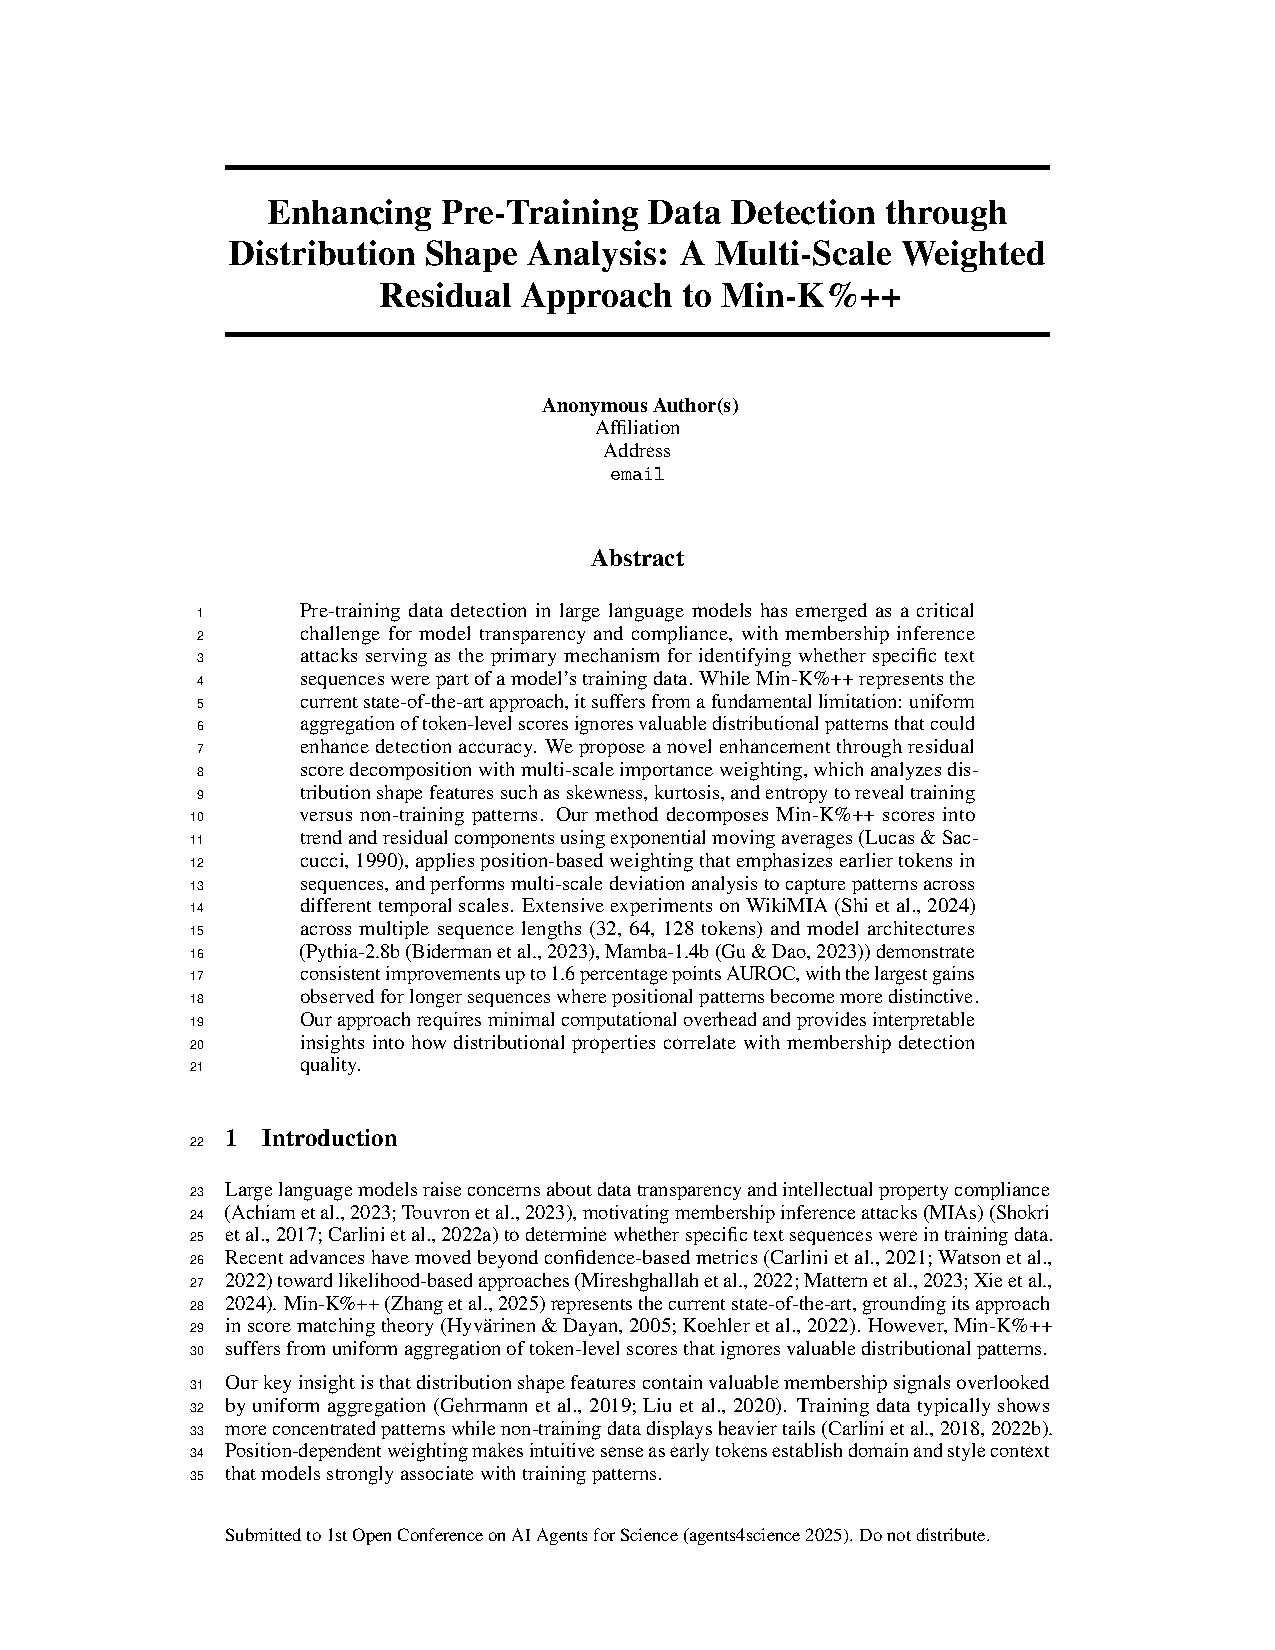
\includepdf[pages=-]{papers/mink++_extended_paper.pdf}

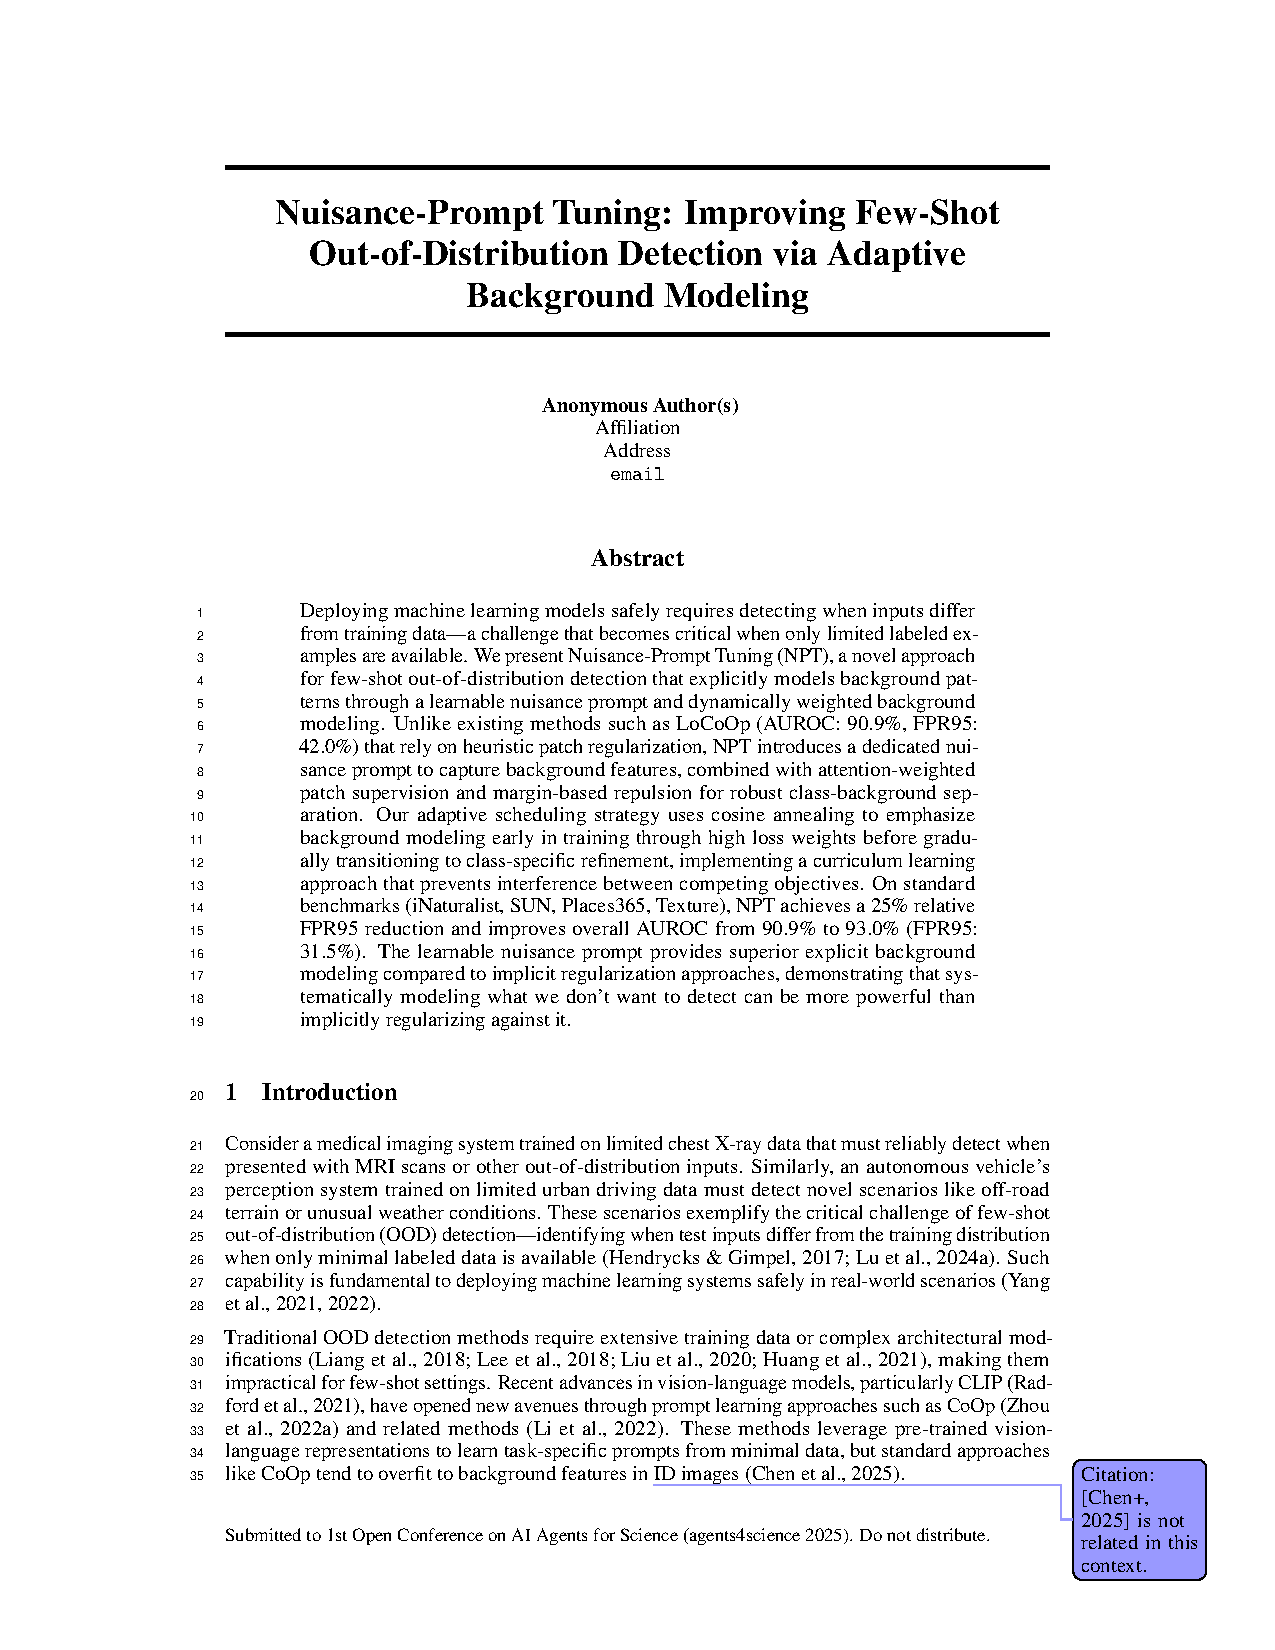
\includepdf[pages=-]{papers/locoop_extended_paper.pdf}

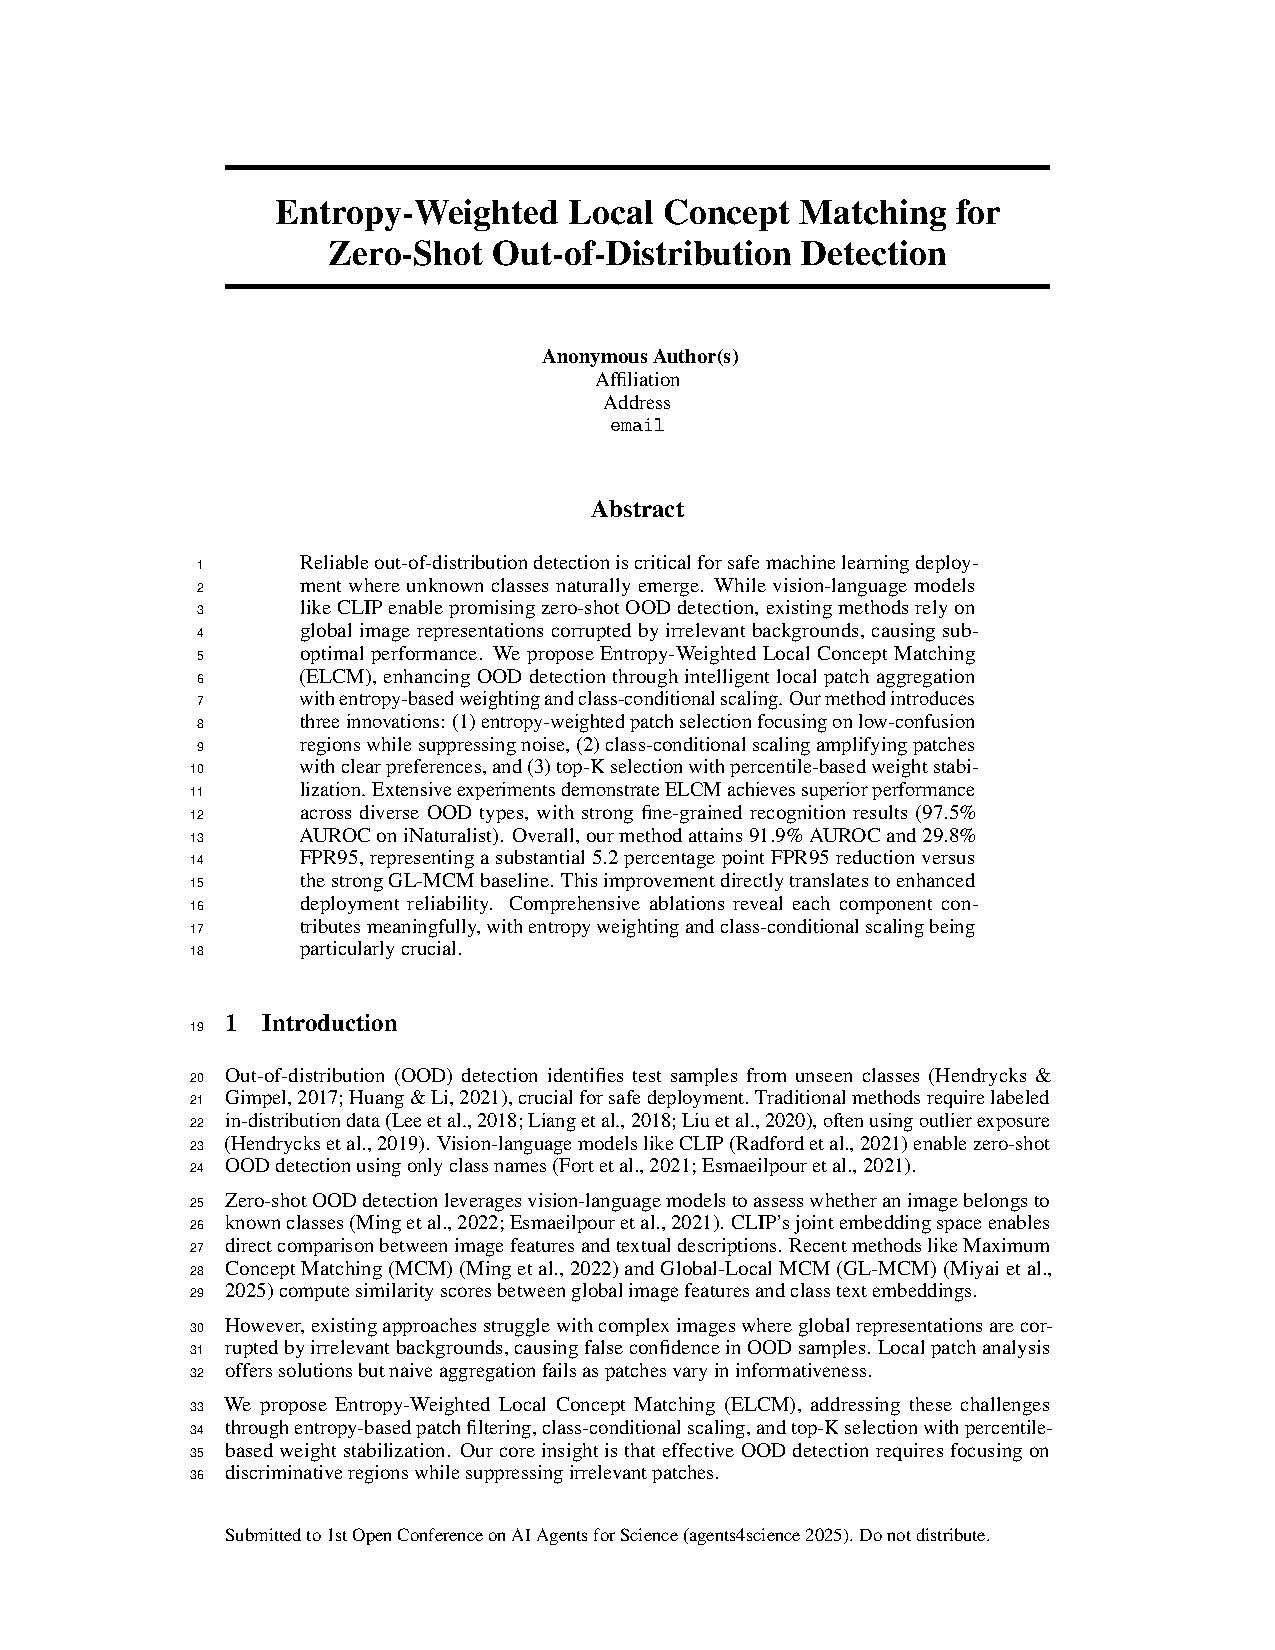
\includepdf[pages=-]{papers/glmcm_extended_paper.pdf}
\let\clearpage\relax